\newpage

\section{Problem description \& Hypothesis}
We belive that we can better manage  the country resouces through the knowldge extracted from data comunications, in this paper the solution is built on the hypotesis of mobility patterns to forecast and manage the resources in a correlated way with the results showns in this paper.
\\
\\
The figure below shows a theoretical commuting model proposed like a main pattern. Two peaks are pointed between 
 
 \begin{figure}[h]
\begin{center}
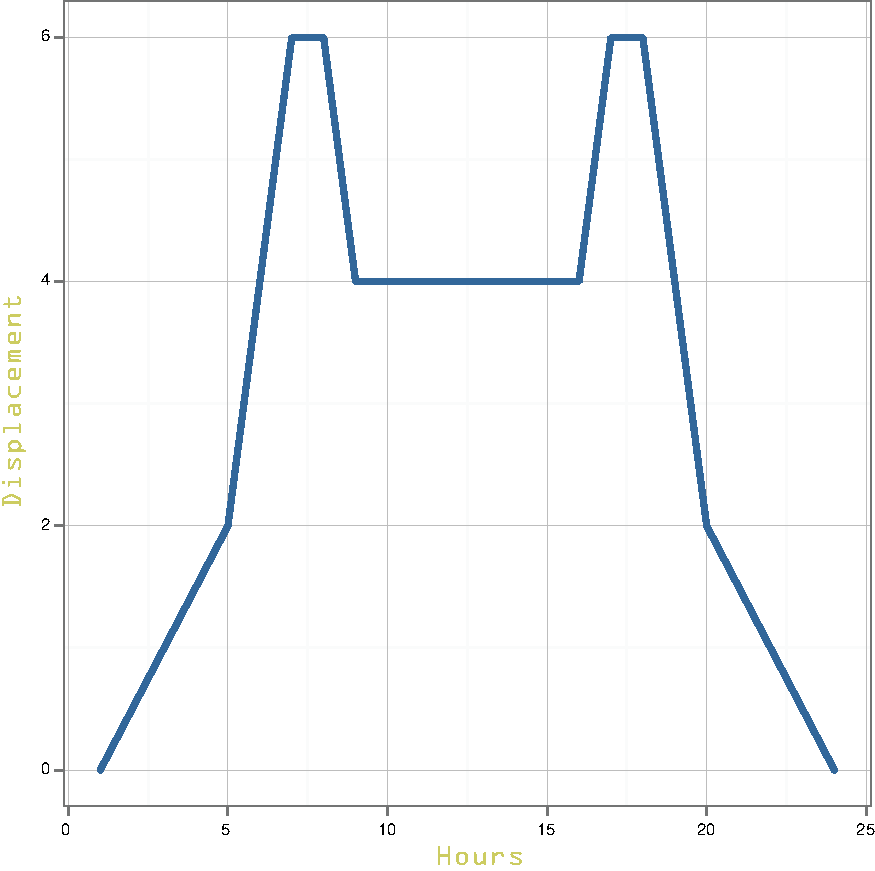
\includegraphics[scale =0.6] {results/images/common_commuting_model.pdf}
\caption{Theoretical Commuting Model}
\label{fig:commuting}
\end{center}
\end{figure}